% Options for packages loaded elsewhere
\PassOptionsToPackage{unicode}{hyperref}
\PassOptionsToPackage{hyphens}{url}
\PassOptionsToPackage{dvipsnames,svgnames,x11names}{xcolor}
%
\documentclass[
  11pt,
]{book}
\usepackage{amsmath,amssymb}
\usepackage{lmodern}
\usepackage{iftex}
\ifPDFTeX
  \usepackage[T1]{fontenc}
  \usepackage[utf8]{inputenc}
  \usepackage{textcomp} % provide euro and other symbols
\else % if luatex or xetex
  \usepackage{unicode-math}
  \defaultfontfeatures{Scale=MatchLowercase}
  \defaultfontfeatures[\rmfamily]{Ligatures=TeX,Scale=1}
\fi
% Use upquote if available, for straight quotes in verbatim environments
\IfFileExists{upquote.sty}{\usepackage{upquote}}{}
\IfFileExists{microtype.sty}{% use microtype if available
  \usepackage[]{microtype}
  \UseMicrotypeSet[protrusion]{basicmath} % disable protrusion for tt fonts
}{}
\makeatletter
\@ifundefined{KOMAClassName}{% if non-KOMA class
  \IfFileExists{parskip.sty}{%
    \usepackage{parskip}
  }{% else
    \setlength{\parindent}{0pt}
    \setlength{\parskip}{6pt plus 2pt minus 1pt}}
}{% if KOMA class
  \KOMAoptions{parskip=half}}
\makeatother
\usepackage{xcolor}
\IfFileExists{xurl.sty}{\usepackage{xurl}}{} % add URL line breaks if available
\IfFileExists{bookmark.sty}{\usepackage{bookmark}}{\usepackage{hyperref}}
\hypersetup{
  pdftitle={Transforming Research Methods in Health Services Psychology: Applications for the Advocate \textasciitilde{} Practitioner \textasciitilde{} Scientist},
  pdfauthor={Lynette H. Bikos, PhD, ABPP \& Cirlene DeBlaere, PhD, Editors; Kiana Clay, Editorial Assistant},
  colorlinks=true,
  linkcolor={Maroon},
  filecolor={Maroon},
  citecolor={Blue},
  urlcolor={blue},
  pdfcreator={LaTeX via pandoc}}
\urlstyle{same} % disable monospaced font for URLs
\usepackage[margin=1in]{geometry}
\usepackage{longtable,booktabs,array}
\usepackage{calc} % for calculating minipage widths
% Correct order of tables after \paragraph or \subparagraph
\usepackage{etoolbox}
\makeatletter
\patchcmd\longtable{\par}{\if@noskipsec\mbox{}\fi\par}{}{}
\makeatother
% Allow footnotes in longtable head/foot
\IfFileExists{footnotehyper.sty}{\usepackage{footnotehyper}}{\usepackage{footnote}}
\makesavenoteenv{longtable}
\usepackage{graphicx}
\makeatletter
\def\maxwidth{\ifdim\Gin@nat@width>\linewidth\linewidth\else\Gin@nat@width\fi}
\def\maxheight{\ifdim\Gin@nat@height>\textheight\textheight\else\Gin@nat@height\fi}
\makeatother
% Scale images if necessary, so that they will not overflow the page
% margins by default, and it is still possible to overwrite the defaults
% using explicit options in \includegraphics[width, height, ...]{}
\setkeys{Gin}{width=\maxwidth,height=\maxheight,keepaspectratio}
% Set default figure placement to htbp
\makeatletter
\def\fps@figure{htbp}
\makeatother
\setlength{\emergencystretch}{3em} % prevent overfull lines
\providecommand{\tightlist}{%
  \setlength{\itemsep}{0pt}\setlength{\parskip}{0pt}}
\setcounter{secnumdepth}{5}
\usepackage{booktabs}
\ifLuaTeX
  \usepackage{selnolig}  % disable illegal ligatures
\fi
\usepackage[]{natbib}
\bibliographystyle{plainnat}

\title{Transforming Research Methods in Health Services Psychology: Applications for the Advocate \textasciitilde{} Practitioner \textasciitilde{} Scientist}
\author{Lynette H. Bikos, PhD, ABPP \& Cirlene DeBlaere, PhD, Editors \and Kiana Clay, Editorial Assistant}
\date{22 Jul 2022}

\begin{document}
\maketitle

{
\hypersetup{linkcolor=}
\setcounter{tocdepth}{3}
\tableofcontents
}
\hypertarget{book-cover}{%
\chapter*{BOOK COVER}\label{book-cover}}
\addcontentsline{toc}{chapter}{BOOK COVER}

\begin{figure}
\centering
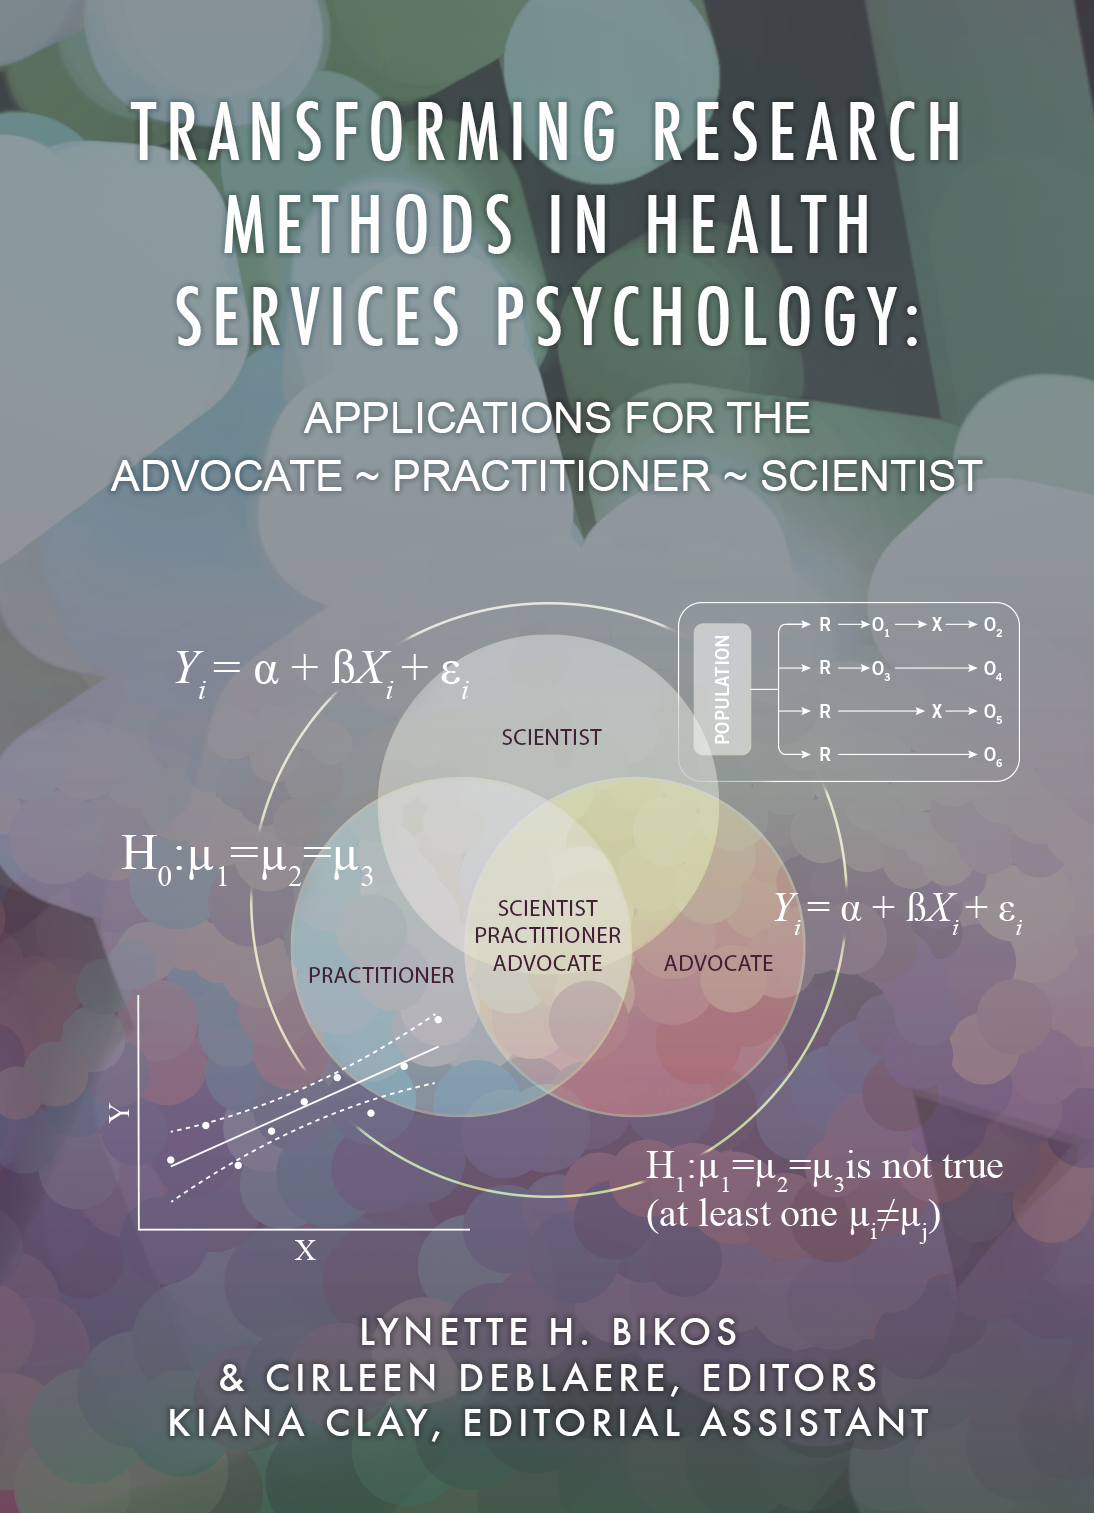
\includegraphics{images/bookcover.png}
\caption{An image of the book cover. It includes three overlapping, pastel-colored, circles representing advocacy, practice, and science. These are surrounded by a handful of statistical symbols and formulae. methods.}
\end{figure}

This open education resource is available in the following formats, all available in the \href{https://github.com/lhbikos/TransformingResearchMethods/tree/main/docs}{docs} folder at the GitHub repository:

\begin{itemize}
\tightlist
\item
  Formatted as an \href{https://lhbikos.github.io/TransformingResearchMethods/}{html book} via GitHub Pages available
\item
  As a \href{https://github.com/lhbikos/TransformingResearchMethods/blob/main/docs/TransformingResearchMethods.pdf}{PDF}
\item
  As an \href{https://github.com/lhbikos/TransformingResearchMethods/blob/main/docs/TransformingResearchMethods.epub}{ebook}
\item
  As a \href{https://github.com/lhbikos/TransformingResearchMethods/blob/main/docs/TransformingResearchMethods.docx}{Word Document}
\end{itemize}

All materials used in creating this OER are available at its \href{https://github.com/lhbikos/TransformingResearchMethods}{GitHub repo}.

\hypertarget{preface}{%
\chapter*{PREFACE}\label{preface}}
\addcontentsline{toc}{chapter}{PREFACE}

\textbf{If you are viewing this document, you should know that this is a book-in-progress. Early drafts are released for the Transforming Counseling Psychology Curriculum Showcase at APA 2022, for peer review, and for generating interest in collaboration. The document was last updated on 22 Jul 2022}.

In her 2021-2022 term as President of the Society of Counseling Psychology, one of Dr.~Amy Reynolds' Presidential Initiatives was \emph{Transforming Counseling Psychology Curriculum and Praxis.} Dr.~Reynolds invited counseling psychology faculty, practitioners, and doctoral students ``to critically examine and deconstruct how various competencies, courses, and content are taught; how we socialize our students; and then re-imagine, dream, and reconstruct new and transformative ways to teach and train.''

\hypertarget{strategies-for-a-social-responsivity}{%
\section*{Strategies for a Social Responsivity}\label{strategies-for-a-social-responsivity}}
\addcontentsline{toc}{section}{Strategies for a Social Responsivity}

This open education resource (OER) is a product of the group devoted to \emph{research}. There are a number of strategies we used to ensure that the OER moves in the direction of being socially and culturally responsive.

\begin{itemize}
\tightlist
\item
  Our authors committed to using the guidelines for a liberated syllabus found in the CCTC: Social Responsiveness in \href{https://pr4tb8rrj317wdwt3xlafg2p-wpengine.netdna-ssl.com/wp-content/uploads/2021/05/CCTC_Socially-Responsive-HSP-Ed-Training_v7.pdf}{Health Services Psychology Education \& Training Toolkit}.
\item
  We chose the format of OER because provides a zero-cost \emph{textbook} to faculty and students.
\item
  We sought authors and co-author teams that represent the diversity of health services psychology including discipline (counseling, clinical, educational),stage in career (students, early career professionals, mid- and late- career professionals), and identities that have been marginalized in higher education and our discipline.
\item
  Each chapter works its way through an open peer review process where the chapter (with authors clearly identified)is hosted in a shared drive. At least two reviewers can mark up the same document and contribute to the same rubric. At any time the author(s) can see the review and, if desired, dialogue with the reviewers. At the outset, we specified the tone to be ``formative not summative.''
\item
  Although we are still learning, we have attempted to use tools and techniques that are consistent with universal design. For example, we hope that the image captions and headers are marked such that text readers will identify them as such.
\end{itemize}

\hypertarget{perpetually-in-progress}{%
\section*{Perpetually in Progress}\label{perpetually-in-progress}}
\addcontentsline{toc}{section}{Perpetually in Progress}

This book is being formatted in R Markdown, rendered into its ``book'' format with Bookdown, hosted on GitHub, and pushed to the internet (in its html format) through GitHub Pages. This set of tools allows the book to be \emph{perpetually-in-progress.} This means that our authors can update their chapters at-any-time. It also means that we can add chapters at-any-time. If you are interested in contributing to the book, please contact us. It is one of our greatest hopes that this flexibility contributes to the socially and culturally responsive pedagogy that we intend.

\hypertarget{under-construction}{%
\section*{Under Construction}\label{under-construction}}
\addcontentsline{toc}{section}{Under Construction}

At this stage in the OER's development, authors are still writing and revising chapters. The following designations will identify the chapters that have not been through the review process:

\begin{itemize}
\tightlist
\item
  \emph{In-progress} means that the chapter is partially written (or perhaps outlined) and that the author(s) are continuing to work on the chapter.
\item
  \emph{Under review} means that the chapter is being (or has been) peer-reviewed.
\end{itemize}

\hypertarget{acknowledgements}{%
\section*{Acknowledgements}\label{acknowledgements}}
\addcontentsline{toc}{section}{Acknowledgements}

Financial support, supporting the copy editing and desktop publishing for this project was provided by the Office of Education, Technology, \& Media, Seattle Pacific University (Summer 2022).

\hypertarget{copyright-with-open-access}{%
\section*{Copyright with Open Access}\label{copyright-with-open-access}}
\addcontentsline{toc}{section}{Copyright with Open Access}

This book is published under a a Creative Commons Attribution-NonCommercial-ShareAlike 4.0 International License. This means that this book can be reused, remixed, retained, revised and redistributed (including commercially) as long as appropriate credit is given to the authors. If you remix, or modify the original version of this open textbook, you must redistribute all versions of this open textbook under the same license - CC BY-SA.

A \href{https://github.com/lhbikos/ReC_MultivModel}{GitHub open-source repository} contains all of the text and source code for the book, including data and images.

\hypertarget{writing-empirical-manuscripts}{%
\chapter*{WRITING EMPIRICAL MANUSCRIPTS}\label{writing-empirical-manuscripts}}
\addcontentsline{toc}{chapter}{WRITING EMPIRICAL MANUSCRIPTS}

\hypertarget{APAstyle}{%
\chapter{The APA Style Manuscript}\label{APAstyle}}

\emph{Lynette H. Bikos (she/her) \& Kiana Clay (she/her)}\\
\emph{Seattle Pacific University}\\
\emph{Seattle Pacific University was built on the unceded ancestral lands of the Duwamish people}\\
Chapter Status: In Progress/Placeholder

This is sample text as we learn how to use the Github.
Ridiculous sentence on line 14. Another ridiculous line to volley it back.

This lesson focuses on APA style. While a significant portion of the material focuses on the mechanics of APA style, I also consider:

\begin{itemize}
\tightlist
\item
  APA style as epistemology -- and its relationship with power, privilege, and racism.
\item
  JARS: Journal Article Reporting Standards
\item
  Section by section
\item
  Consideration of writing as a developmental process that occurs throughout grad school and into the profession
\item
  Stylistic issues
\item
  Hallmarks of APA style
\item
  Reducing bias
\end{itemize}

\hypertarget{navigating-this-lesson}{%
\section{Navigating this Lesson}\label{navigating-this-lesson}}

There is about 1 hour and 45 minutes of lecture.

The R markdown file used to create this lecture as well as all of the figures are available at the \href{https://github.com/lhbikos/ReC_Topics}{OER's GitHub site}.

\hypertarget{learning-objectives}{%
\subsection{Learning Objectives}\label{learning-objectives}}

Learning objectives from this lecture include the following:

\begin{itemize}
\tightlist
\item
  Identify the cultural characteristics of APA style.
\item
  Identify two ways that Thompson (2004) has suggested that APA style perpetuates Whiteness and patriarchy in the academy.
\item
  List the components of an abstract.
\item
  Describe why JARS matters.
\item
  Begin memorizing the minutia of APA Style for writing empirical manuscripts/journal articles (no particular order).
\end{itemize}

\hypertarget{readings-resources}{%
\subsection{Readings \& Resources}\label{readings-resources}}

In preparing this chapter, I drew heavily from the following resource(s). Other resources are cited (when possible, linked) in the text with complete citations in the reference list.

\begin{itemize}
\tightlist
\item
  American Psychological Association. (2020). \emph{Publication manual of the American Psychological Association: The official guide to APA style. (Seventh edition.).} American Psychological Association.

  \begin{itemize}
  \tightlist
  \item
    I'm guessing you'll use this more days than not, for the rest of your education.
  \end{itemize}
\item
  Tran, A. G. T. T., \& Lee, R. M. (2014). You speak English well! Asian Americans' reactions to an exceptionalizing stereotype. \emph{Journal of Counseling Psychology, 61}(3), 484--490. \url{https://doi.org/10.1037/cou0000034}

  \begin{itemize}
  \tightlist
  \item
    I use this article in several analyses in the ANOVA series as well as in this lesson when I compare/contrast it to the requirements of APA Style. This article was pubbed in 2014; but I will compare it to the 7th edition (2019) standards.
  \end{itemize}
\item
  Cooper, H. (2020). \emph{Reporting quantitative research in psychology: How to meet APA style journal article reporting standards (Second edition, revised.).} American Psychological Association. \url{https://alliance-primo.hosted.exlibrisgroup.com/permalink/f/rpqmv/CP71332049420001451}

  \begin{itemize}
  \tightlist
  \item
    The e-text version of this may be available at your library. This resource offers section-by-section instruction of the reporting standards and provides numerous examples of writing APA empirical manuscripts.
  \end{itemize}
\item
  Madigan, R., Johnson, S., \& Linton, P. (1995). The language of psychology: APA style as epistemology. American Psychologist, 50(6), 428--436. \url{https://doi.org/10.1037/0003-066X.50.6.428}

  \begin{itemize}
  \tightlist
  \item
    Madigan et al.~(1995) argued that as we learn APA style we are inculcating the professional values of our discipline (and we do this without awareness).
  \end{itemize}
\item
  Thompson, A. (2004). Gentlemanly Orthodoxy: Critical Race Feminism, Whiteness Theory, and the APA Manual. \emph{Educational Theory, 54}(1), 27--57. \url{https://doi.org/10.1111/j.0013-2004.2004.00002.x}
\item
  Critiquing the 5th edition of the style manual (we're now on the 7th) Thompson (2004) pointed out how aspects of APA style contribute to preserving Whiteness.
\item
  Appelbaum, M., Cooper, H., Kline, R. B., Mayo-Wilson, E., Nezu, A. M., \& Rao, S. M. (2018). Journal article reporting standards for quantitative research in psychology: The APA Publications and Communications Board task force report. \emph{American Psychologist, 73}(1), 3--25. \url{https://doi.org/10.1037/amp0000191}

  \begin{itemize}
  \tightlist
  \item
    Yet another copy of the most current JARS. You can also find them in the style manual and on their own website: \url{https://apastyle.apa.org/jars/glossary}
  \end{itemize}
\item
  \emph{White Supremacy Culture.} (n.d.). DRworksBook. Retrieved August 8, 2020, from \url{https://www.dismantlingracism.org/white-supremacy-culture.html}

  \begin{itemize}
  \tightlist
  \item
    Identifies characteristics of White Supremacy Culture in organizations (often used to describe academia).
  \end{itemize}
\end{itemize}

\hypertarget{apa-style-as-epistemology-or-worse}{%
\section{APA Style as Epistemology (or Worse)}\label{apa-style-as-epistemology-or-worse}}

A 1995 article \citep{madigan_language_1995} in the American Psychologist compared APA style to that of other disciplines (history, literary criticism) and argued that APA Style is its own writing genre characterized by (among other things):

\begin{itemize}
\tightlist
\item
  A story schema: introduction, method, results, discussion
  -- Seems so linear; but this is rarely the case (research is messy). This schema serves as an implicit formula for addressing psychological questions:
\end{itemize}

\begin{enumerate}
\def\labelenumi{\arabic{enumi})}
\tightlist
\item
  Review of past empirical studies
\item
  Collection and analysis of new data
\item
  Relation of conclusions to current psychological theories
\end{enumerate}

\begin{itemize}
\tightlist
\item
  A depersonalized language of disagreement that focuses on the empirical process and away from investigators as individuals (e.g., ``The primary criticism is that the threshold-setting procedures used in previous experiments are not adequate to ensure that\ldots{}''). The goal is a collaborative, cumulative endeavor based on research data that avoids animosity and confrontation.
\item
  Hedged conclusions: balancing a need to have substantive conclusions that do not extend beyond the data. We use the words, ``tend,'' ``suggest,'' and ``may'' (see Table 1) to allow authors to relate findings, while still recognizing the need for additional research before asserting firm conclusions. **NOTE: INCLUDE TABLE 1!!!
\item
  A system of headings/subheadings (rather than narrative transitions)
\item
  Paraphrasing rather than directly quoting other works.
  -- Giving authors more flexibility in representing others' perspectives.
\item
  Multiple authors (perhaps contributing to ``more subdued prose'').
\item
  Heavy use of citations in the introduction and discussion sections so that the research is placed within an ongoing stream of empirical studies. The use of in-text references provides vital background for the study and helps the author establish credibility as an expert on the subject they are researching.
\item
  Language that ``does not call attention to itself.'' It can be described as: self-effacing and low-profile. Colorful language and attention-grabbing metaphors are rarely used; the focus is meant to be on the phenomena being studied.
\end{itemize}

The style manual has grown from its 7-page writers guide in the Psychological Bulletin (1929) to 427 in the 7th edition (2019), today. Madigan et al. \citeyearpar{madigan_language_1995} suggests that the process of mastering APA style, one is enculturated into psychology. That is, we learn APA style -- we inculcate empiricist values (i.e., ``unarticulated practices that reflect fundamental attitudes and values of psychologists'' (p.~428). As such, APA style is epistemological.

Nearly a decade later, Thompson \citeyearpar{thompson_gentlemanly_2004} examined APA style through the lens of critical race feminism and Whiteness Theory. Thompson argued that the expectations regarding clarity precision, appropriateness, sensitivity, and objectivity likely contribute to the academy's investments in Whiteness and patriarchy. While her focus was on APA Style, she suspected that her critique would generalize to other style guides (e.g., Chicago, MLA).

Thompson's \citeyearpar{thompson_gentlemanly_2004} article focused around the gender/sexuality and race values codified by the APA manual (at the time of her article it was the 5th edition). She conducted an analysis of its \emph{power and property investments} and organized her arguments in five themes:

\textbf{Property Rights}: PWIs have treated refereed scholarship (but not indigenous or community knowledge) as intellectual property, demarcated with a certain class. That is, individuals ``own knowledge.'' Evidence includes:

\begin{itemize}
\tightlist
\item
  Using last names as a shorthand reference for work (e.g., ``Dik \& Duffy's 2012 CVQ'').
\item
  Tendency to cite own work rather than say, ``When I previously said\ldots{}''
\item
  The style manual indicates that principal authorship and order of authorship credit should reflect the relative contributions of persons involved (7th ed, APA 1.22) and that relative status should not determine authorship order. Thompson argued that power dynamics (especially around race and gender) likely interfere with this principle.
\item
  The 7th edition has reduced citations of articles with three and more articles to ``First author et al., YEAR'' for all citations.\\
\item
  Regarding, ownership of knowledge -- does it belong to the researcher or the community from which it came? Community knowledge can be studied but not cited. And what about institutions? What if knowledge came from the Black Church? How does one cite that?
\end{itemize}

\textbf{Precedent and pedigree}: In the social sciences, we are expected to cite and give credit to relevant earlier works. Knowledge is seen as cumulative. Citations are essential.

\begin{itemize}
\tightlist
\item
  No ``unhedged statement'' (p.~45) is made without a citation; and in introductory sections, citations are often included with claims that seem obvious! This establishes the requisite lineage.
\item
  Self-citations, expected citations (of the gurus), citations of colleagues exist IN TENSION with a citation economy (page limits, after all).
\item
  The requirement that scholars locate their project in the context of the existing peer-reviewed literature serves to keep out ideas/projects that would be challenging to the existing power structure.
\end{itemize}

\textbf{Proceduralism}: APA authors learn to address an audience unmarked (as if they were white, male, heterosexual) by gender or race as a ``sign of professionalism'' (p.~48).

\begin{itemize}
\tightlist
\item
  Standardized Format: a four section structure: Introduction, Method, Results Discussion; it could be that the experiences of marginalized and oppressed groups cannot be captured by this scientific narrative structure.
\item
  Standardized Style: prizing scientific appearance and elegance. Thompson (2004) follows the guidelines regarding the use of the ``slash'' (/) and how it is impossible to standardize to the degree that it works for all groups.

  \begin{itemize}
  \tightlist
  \item
    The ``First author et al., (year)'' citation contributes to both gender- and color-blindness. On the one hand is it ``fair.'' On the other hand, it obscures the person of the author.
  \item
    APA's prohibition against footnotes minimizes ``the good stuff'' (the most juicy arguments are always in the footnotes).
  \end{itemize}
\end{itemize}

\textbf{Protocol}: Propriety or protocol represents conduct that signifies one's understanding of prevailing relations of power, authority and legitimacy.

\begin{itemize}
\tightlist
\item
  The style manual (7th ed, Chapter 5, e.g., 5.2) acknowledges the importance of sensitivity and the avoidance of pejoratives to reference groups of people. Thompson indicates that this is ``admirable'' it fails to address unequal power relations. Further, distinctions between what is insensitive and pejorative may be invisible to those in positions of privilege.
\end{itemize}

\textbf{The gentleman's agreement}: APA style is characterized ``language that conveys professionalism and formality'' (7th ed, 4.7, 4.8) and ``differences should be presented in a professional and noncombative manner'' (7th ed, 4.7).

\begin{itemize}
\tightlist
\item
  Thompson \citeyearpar{thompson_gentlemanly_2004} is concerned that while this is offered with the hope of pluralism and the creation of safe spaces, it causes controversies to be ignored or dismissed and may bolster complicity in racism.
\end{itemize}

\hypertarget{as-we-dive-into-the-specifics}{%
\section{As We Dive into the Specifics}\label{as-we-dive-into-the-specifics}}

Please keep the perspectives of these authors in mind.

Let's also look at the characteristics of White Supremacy Culture in organizations \citep{noauthor_white_nodate}. As we tour through the components of APA style, what resonates with this list? Refer to the .pdf handout or website for more definitions, descriptions, examples, and antidotes.

\begin{itemize}
\tightlist
\item
  Perfectionism

  \begin{itemize}
  \tightlist
  \item
    Perfectionistic culture
  \item
    Worship of the written word
  \item
    Only one right way
  \item
    Either/or thinking
  \end{itemize}
\item
  Concentration of power

  \begin{itemize}
  \tightlist
  \item
    Power hoarding
  \end{itemize}
\item
  Paternalism

  \begin{itemize}
  \tightlist
  \item
    Defensiveness
  \end{itemize}
\item
  Right to comfort

  \begin{itemize}
  \tightlist
  \item
    Fear of open conflict
  \end{itemize}
\item
  Individualism

  \begin{itemize}
  \tightlist
  \item
    I'm the only one
  \end{itemize}
\item
  Progress is more/bigger

  \begin{itemize}
  \tightlist
  \item
    Objectivity
  \item
    Quantity over quality
  \item
    Sense of urgency
  \end{itemize}
\end{itemize}

\hypertarget{the-jars-the-core-of-apa-style}{%
\section{The JARS: The Core of APA Style}\label{the-jars-the-core-of-apa-style}}

The JARS {[}Journal Article Reporting Standards; \citet{appelbaum_journal_2018}{]} were first introduced in a 2008 feature in the American Psychologist \citep{noauthor_reporting_2008} and were included in the 6th edition of the style manual. The updated JARS, published in 2018, expanded the types of quantitative research (JARS-Quant) and included standards for reporting qualitative (JARS-Qual) and mixed methods (JARS-Mixed). Chapter 3 of the 7th edition is devoted to JARS. It contains numerous tables, definitions/explanations, and a flowchart.

The JARS are an attempt to represent what is common across approaches. There is a recognition that specialties/sub-specialties use different terminology. The terms, therefore, should be treated as placeholders and be updated to reflect the various research traditions.

In each of the sections below, I list both the APA style recommendations and JARS elements -- which are somewhat annoyingly separate, adjacent, and overlapping.

In the next section I used text-citations to also refer to the section numbers of the 7th edition of the APA style manual. Additionally, because this OER is publicly available (i.e., not just used in my classroom), I have not copied the JARS elements into this document. They are freely available \href{https://apastyle.apa.org/jars/quantitative}{here}.

\hypertarget{title-authorship-author-note-apa-2.3}{%
\subsection{Title, Authorship, Author Note (APA 2.3)}\label{title-authorship-author-note-apa-2.3}}

***ARE WE KEEPING THE QUIZLETS? QUIZLET:
A manuscript title should

\begin{enumerate}
\def\labelenumi{\alph{enumi}.}
\tightlist
\item
  Use abbreviations whenever possible
\item
  Contain at least 30 words
\item
  Be fully explanatory when standing alone
\item
  Begin with the words, A Study of
\end{enumerate}

The title page of a manuscript includes the

\begin{enumerate}
\def\labelenumi{\alph{enumi}.}
\tightlist
\item
  Author's name
\item
  Author's institutional affiliation'
\item
  Running head
\item
  Short title
\item
  All of the above
\end{enumerate}

\hypertarget{title-apa-2.4}{%
\subsubsection{Title (APA 2.4)}\label{title-apa-2.4}}

\begin{itemize}
\tightlist
\item
  Concise statement of main topic of the research,
\item
  Identify the variables or theoretical issues under investigation (and the relationship between t Addhem),
\item
  Focused and succinct (no prescribed word or character limit per the style manual; but a journal may have one).
\item
  Avoid empty words/phrases like ``A study of,'' ``An investigation of''
\end{itemize}

\emph{The lecture further reviews JARS elements.}

\hypertarget{authorshipbyline-apa-2.5-affiliation-apa-2.6}{%
\subsubsection{Authorship/Byline (APA 2.5) \& Affiliation (APA 2.6)}\label{authorshipbyline-apa-2.5-affiliation-apa-2.6}}

\begin{itemize}
\tightlist
\item
  Primary contributors;
\item
  Institutional affiliation AT THE TIME of the study, no more than 2 institutional affiliations (and they both need to have contributed equally)
\item
  Very specific style guidelines (with superscript notations) for connecting authors and their affiliations
\item
  In the order of contribution -- lots of ethical, practical, and sensitive considerations about who gets to be an author and in what order.
\end{itemize}

\textbf{Sticky Issues about Authorship}

\begin{itemize}
\tightlist
\item
  Faculty as first authors
\item
  Ongoing projects with years of investment sponsored by faculty
\item
  Who gets ``the call''? (is ``the call'': who gets to decide who is first author?)
\item
  Order between equal contributors (e.g., Singer \& Willett)
\item
  In equal contributions it is okay (but not ideal) to mention in the author note
\item
  GOAL: name on a project, less concerned about author order
\item
  Generally, graduate projects include the faculty sponsor as an author
\item
  Author-order \href{https://github.com/lhbikos/TransformingResearchMethods/blob/main/Authorship\%20Rubric220721.xlsx}{rubrics} can be useful to guide the decision
\end{itemize}

\hypertarget{author-note-apa-2.7}{%
\subsubsection{Author Note (APA 2.7)}\label{author-note-apa-2.7}}

Place the author note at the bottom half of title page. There are more specific instructions in style manual. Generally author note has four paragraphs:

\begin{itemize}
\tightlist
\item
  ORCID iDs \url{https://orcid.org}
\item
  Changes in affiliation subsequent to the time of the study, ``{[}Author's name{]} is now at {[}new affiliation{]}.'' Can also be used if an author is deceased.
\item
  Disclosures and acknowledgements (i.e., study registration, open practices and data sharing, related reports, conflicts of interest, financial or other assistance).
\item
  Contact information for corresponding author. Requires full name, complete mailing address, and e-mail. Prescribed format: Correspondence concerning this article should be addressed to {[}author's name'{]}, {[}complete mailing address{]}. Email: \href{mailto:author@institution.edu}{\nolinkurl{author@institution.edu}}
\end{itemize}

\emph{The lecture further reviews JARS elements.}

\hypertarget{running-head-apa-2.8}{%
\subsubsection{Running Head (APA 2.8)}\label{running-head-apa-2.8}}

\begin{itemize}
\tightlist
\item
  Abbreviated title printed at the top of the pages of a ms or pubbed article to identify it for the readers
\item
  Max of 50 characters (counting letters, punctuation, spaces between words). If the title is already 50 characters or fewer, the full title can be used. Avoid abbreviations in the running head, although the ampersand can be swapped (\& for ``and'').
\item
  Appears flush left in all uppercase letters at the top of the title and subsequent pages
\end{itemize}

\hypertarget{manuscript-page-headerspage-numbers-apa-8.03}{%
\subsubsection{Manuscript Page Headers/Page Numbers (APA 8.03)}\label{manuscript-page-headerspage-numbers-apa-8.03}}

\begin{itemize}
\tightlist
\item
  Number consecutively, beginning with the title
\item
  Identify each page with the running head along with the page number
\item
  To facilitate a blinded review, do not include your name in the page header
\item
  Use the automatic functions of the word-processer to generate page headers and page numbers
\end{itemize}

\hypertarget{abstract-apa-2.8-3.3}{%
\subsection{Abstract (APA 2.8, 3.3)}\label{abstract-apa-2.8-3.3}}

QUIZLET:
An abstract should

\begin{enumerate}
\def\labelenumi{\alph{enumi}.}
\tightlist
\item
  Appear on the same page above the title and introduction
\item
  Be single-spaced and set with larger margins
\item
  Begin on page 2
\item
  Be no longer than 3\% of the text
\end{enumerate}

Abstract lengths vary from journal to journal; the typical range is from \_\_\_ to\_\_\_ words. (250 to 500???)

A good abstract is:

\begin{itemize}
\tightlist
\item
  Concise and specific
\item
  Nonevaluative
\item
  Coherent and readable
\item
  Loaded with keywords
\item
  May be a single paragraph (no indentation of first line) or structured (still no indentation, but labels inserted for the prescribed sections).
\end{itemize}

\hypertarget{recipe-for-an-abstract}{%
\subsubsection{Recipe for an Abstract}\label{recipe-for-an-abstract}}

\begin{itemize}
\tightlist
\item
  Identify the problem under investigation (1 sentence)
\item
  Identify the participants and salient characteristics
\item
  Identify the experimental method, including the apparatus, data gathering procedures, complete test names, etc.
\item
  Identify findings (including statistical significance levels)
\item
  Identify conclusions and implications/applications.
\item
  Avoid \emph{boilerplate} sentences.
  -- At the end of an abstract, I often read, ``Findings and implications will be discussed.'' This is boilerplate because ``everyone says it.'' It's also empty and a waste of words because it tells us NOTHING about the study.
\item
  The style manual includes outlines for a variety of types of manuscripts.
\end{itemize}

\emph{The lecture further reviews JARS elements.}

\hypertarget{keywords}{%
\subsubsection{Keywords}\label{keywords}}

Keywords include single words, phrases, or acronyms that describe the most important aspects of the paper. The purpose is indexing in databases (it's what we search on in database like PsychInfo).

\hypertarget{introduction-apa-2.11}{%
\subsection{Introduction (APA 2.11)}\label{introduction-apa-2.11}}

QUIZLET:
The introduction section of a research report should:

\begin{enumerate}
\def\labelenumi{\alph{enumi}.}
\tightlist
\item
  Include a thorough historical review of the literature
\item
  Define all of the terms that would be unintelligible to a reader with no previous exposure to the field
\item
  Present the specific problem to be explored and described in the research strategy
\item
  Be clearly labeled.
\end{enumerate}

What question should the introduction section of a research report attempt to answer?
a. What are the theoretical implications of the current research?
b. What is the point of the study?
c.~What is the logical link between the problem and the research strategy?
d.~All of the above are correct.
e. Only a and c of the above are correct.

Before you write, consider this:

\begin{itemize}
\tightlist
\item
  Why is this problem important?
\item
  How does this study link to previous work?
\item
  What are the primary/secondary hypotheses/objectives? What are their links to theory?
\item
  How do the hypotheses and research design relate to each other?
\item
  What are the theoretical and practical implications?
\end{itemize}

Three parts to the Introduction

\begin{itemize}
\tightlist
\item
  Brief introduction, 1-2 paragraphs
\item
  Review of relevant scholarship, 1-2 pages
\item
  Purpose, rational, hypotheses, 1-2 paragraph's at the section's close.
\end{itemize}

\hypertarget{the-brief-introduction}{%
\subsubsection{The Brief Introduction}\label{the-brief-introduction}}

A good introduction paragraph answers the following questions in 1-2 paragraphs

\begin{itemize}
\tightlist
\item
  What is the point of the study?
\item
  How do the hypothesis and experimental design relate to the problem?
\item
  What are the theoretical implications of the study and how does the study relate to previous work in the area?
\item
  What are the theoretical propositions tested and how were they derived?
\end{itemize}

In the middle\ldots above ALL

\begin{itemize}
\tightlist
\item
  Demonstrate that the problem is IMPORTANT
\item
  Narrative thread.
\item
  Always refer to the THEORETICAL BACKGROUND
\item
  Narrative thread.
\item
  Closing paragraph a statement of purpose and rationale of project.
\item
  Narrative thread.
\end{itemize}

The closing paragraph(s) of the Introduction

\begin{itemize}
\tightlist
\item
  What variables did I plan to manipulate?
\item
  What results did I expect and why did I expect them? (the logic of this should also be made clear)
\item
  What is my rationale for each hypothesis?
\end{itemize}

\emph{The lecture further reviews JARS elements.}

\hypertarget{bikos-developmental-perspective-on-learning-to-write-the-empirical-manuscript}{%
\subsubsection{Bikos' Developmental Perspective on Learning to Write the Empirical Manuscript}\label{bikos-developmental-perspective-on-learning-to-write-the-empirical-manuscript}}

Over the years I have been learning writing skills of my own and, in my roles as instructor and peer reviewer, providing feedback to others. Below is an oversimplified model of what I think I'm observing as students and scholars learn to write empirical manuscripts (in the specific APA style).

Figure 1. The first stage of writing.

\begin{figure}
\centering
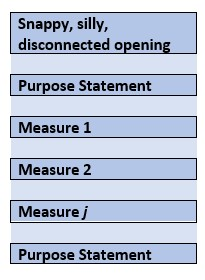
\includegraphics{images/APAstyle/Stage1.jpg}
\caption{Image of the first stage of writing}
\end{figure}

Figure 2. The second stage of writing.

\begin{figure}
\centering
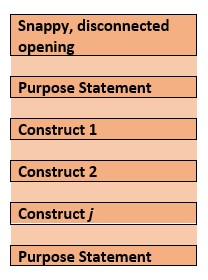
\includegraphics{images/APAstyle/Stage2.jpg}
\caption{Image of the second stage of writing}
\end{figure}

Figure 3. The third stage of writing.

\begin{figure}
\centering
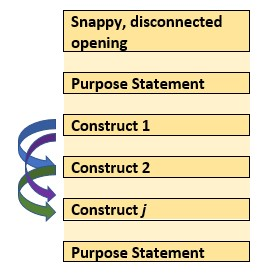
\includegraphics{images/APAstyle/Stage3.jpg}
\caption{Image of the third stage of writing}
\end{figure}

Figure 4. The fourth stage of writing.

\begin{figure}
\centering
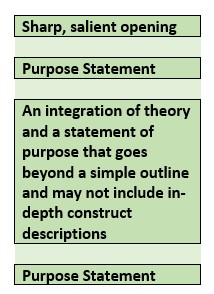
\includegraphics{images/APAstyle/Stage4.jpg}
\caption{Image of the fourth stage of writing}
\end{figure}

\hypertarget{perennial-notes-from-research-project-faculty-graders}{%
\subsubsection{Perennial Notes from Research-Project Faculty Graders}\label{perennial-notes-from-research-project-faculty-graders}}

\begin{itemize}
\tightlist
\item
  Start with your problem statement
  -- What is your DV and why does the reader care?
\item
  Theory must drive your model/manuscript.
  -- ``A list of variables does not a theory-driven model make.''
\item
  Active headers are your friends
  -- Not helpful: ``Gender \& RSB''
  -- More helpful: ``RSB vary across Genders''
\end{itemize}

\hypertarget{method-apa-2.06-chapter-3}{%
\subsection{Method (APA 2.06; Chapter 3)}\label{method-apa-2.06-chapter-3}}

\begin{itemize}
\tightlist
\item
  Describes in detail how the study was conducted.
\item
  Includes conceptual and operational definitions of variables.
\item
  How much info is enough? Readers must be able to\ldots{}
  -- Evaluate the appropriateness of the method
  -- Judge the reliability and validity of your results
  -- Replicate the study
\end{itemize}

Many of the JARS elements have even more detail in the text that follows the table. In your first few papers, make sure to review and imitate.

\emph{The lecture further reviews JARS elements.}

Regarding these tables -- flowchart and tables in style manual, Appelbaum (2018) article, or \href{https://apastyle.apa.org/jars/jars-quant-decision-flowchart.pdf}{website}.

\hypertarget{results-discussion-chapter-3}{%
\subsection{Results \& Discussion (Chapter 3)}\label{results-discussion-chapter-3}}

\emph{The lecture references the JARS elements in detail.}

Section 6.43 of the APA style manual details the basic form for statistical output (``statistical strings''); 6.44 provides statistical abbreviations and symbols.

\hypertarget{headings-apa-2.7}{%
\subsection{Headings (APA 2.7)}\label{headings-apa-2.7}}

The 7th edition of the style manual updated the levels of headings. The change is to the L3 heading -- making it a little easier for Word processing programs.

There are now 5 levels of headings. A useful table that illustrates them can be found \href{https://apastyle.apa.org/style-grammar-guidelines/paper-format/headings}{here}.

Headings follow a top-down progression.

\begin{itemize}
\tightlist
\item
  Each section (i.e., Title {[}on first page{]}, Method, Results, Discussion) starts with an L2 heading.
\item
  Do not include an ``Introduction'' heading -- the first paragraphs of a paper are automatically expected to be introductory in nature.
  Here's the heading structure in the paper (a ``brief report'') we are investigating:
\end{itemize}

\textbf{You Speak English Well! Asian American's Reactions to an Exceptionalizing Stereotype Microaggressions Against Asian Americans} (L1, centered, bold, title case)

\textbf{Method} (L1, centered, bold, title case)

\textbf{Sample} (L2, flush left, bold, title case)
\textbf{Procedure and Materials} (L2, flush left, bold, title case)
\textbf{Analysis and Manipulation Check} (L2, flush left, bold, title case)

\textbf{Results} (L1, centered, bold, title case)

\textbf{Discussion} (L1, centered, bold, title case)

\textbf{Conclusion} (L1, centered, bold, title case)

\hypertarget{reference-list}{%
\subsection{Reference List}\label{reference-list}}

The reference list should start on a new page with ``References'' in bold and centered (an L1 heading -- like the title).

The general format of the reference is: Author (Date). Title. Source. The 7th edition has made significant improvements in making this format consistent throughout the many types of references. Plus, Chapter 9 in the 7th edition has a number of tools for problematic reference entries.

One substantial change in the 7th edition is the immediate use of ``et al.'' after the first author's name when there are three or more authors. In contrast, up to 20 authors can be included in the entry in the reference list.

Use a hanging indent and format this with the paragraph-formatting function of your word processor's ruler. This means that the first line of each reference is flush left and subsequent lines are indented by 0.5 inches.

The text-citations and reference lists must be 100\% consistent. If you have consistently (and properly) used your reference management system, this will happen by magic. Even so, one of the last things I do is a text-ref/ref-list cross check. I open 2 copies of the manuscript and put them side-by-side on the monitor. Starting with the text (and in track changes), each time I come to a reference, I put an X in front of it on the reference list. I go through the entire document. If there are items in the reference list missing, I note it, and then add it. If there are additional references in the reference list that I have not checked, I do a quick search to see if they are really missing, and if so, I delete them. ****SHOULD THIS PART BE KEPT? For dissertation proposals and defenses, we ask first and second year students to do this for us -- it familiarizes them with RVT topics, the dissertation process, and the literature.

Because of Zotero, Mendeley, RefWorks, EndNote, and other reference management systems (as well as the good tools in the style manual), I won't say more about text-citations and reference lists.

\hypertarget{stylistic-issues-apa-chapter-4-on-writing-style-and-grammar}{%
\subsection{\texorpdfstring{Stylistic Issues (APA Chapter 4 on \emph{Writing Style and Grammar})}{Stylistic Issues (APA Chapter 4 on Writing Style and Grammar)}}\label{stylistic-issues-apa-chapter-4-on-writing-style-and-grammar}}

APA (4.0) is committed to a literary style characterized by continuity (logical consistency of expression throughout a written work), flow (smooth cadence of words and sentences), conciseness (say only what you need to say), and clarity. I encourage the authors to read Chapter 4 of the style manual for examples of how to increase the effectiveness with which they write.

\begin{itemize}
\tightlist
\item
  Transitional words between sentences and phrases (or sentences) between paragraphs and sections assist with continuity and flow
  -- Time: then, next, after, while, since
  -- Cause-effect: therefore, consequently, as a result
  -- Addition links: in addition, moreover, furthermore, similarly
  -- Contrast links: but, conversely, nevertheless, however, although
  -- Think twice about using adverbs (certainly, consequently, importantly, interestingly) as transition words.
\item
  Active headings/subheadings contribute to continuity and flow.
\item
  Don't add any more words than necessary. Say \emph{only} what needs to be said:
  -- No ``fluff'' (avoid: very, really)
  -- Maintain a professional tone (avoid cliché's, rhymes, alliteration, metaphors, slang -- remember a global audience)
\item
  Clarity is improved with a varied sentence length; long sentences can be confusing.
\item
  APA style permits both active (subject, verb, object: ``students completed surveys) and passive (object of verb is presented first: ``surveys were completed by students'') voice. The active voice contributes to direct, clear, and concise statements.
\end{itemize}

More style-congruent advice:
* Avoid abstract stacking.
* Avoid organizing by an author(s)' name(s).
-- Organize by ideas -- Unless it is important, citations should be at the end of a sentence. Ask yourself why you are starting a sentence with an author's name -- Is he or she the point of your sentence? Could be but most likely not.
* Use quotations sparingly: short ones, infrequently.
* Precision, continuity, clarity, efficiency (stop with the long sentences)
* Active voice (``It'' is banned as first word in paragraphs and sentences).
* Manuscript must be written in first person.
-- Avoid this: ``Hypotheses for the present study included\ldots{}''
-- Do this instead: ``In our study, we hypothesized\ldots{}''
* Past tense or present perfect tense for the literature review, method, and results sections; present tense for the discussion section.

\hypertarget{reducing-bias-apa-chapter-5}{%
\subsection{Reducing Bias (APA Chapter 5)}\label{reducing-bias-apa-chapter-5}}

Chapter 5, ``Bias-Free Language Guidelines'' is new to the 7th edition. A big message is that this is-and-will-continue-to-be-evolving.

Here are some of the highlights

\begin{itemize}
\tightlist
\item
  Describe relevant characteristics; it is likely unnecessary to collect and/or report on all personal characteristics for the topic being explored.
\item
  Do not shy away/hide/gloss over actual differences in the target population from the general population. Describe them clearly and professionally.
\item
  There are specific guidelines for level of specificity in labels/language for various topics (e.g., disability, age, gender identity, race/ethnicity/nationality, sexual orientation, SES). Look them up.
\item
  A few guiding principles (but there are so many more\ldots read the chapter):
  -- Call people what they call themselves (especially in qualitative or participant-informed research designs). Also recognize that no group is monolithic so there may be within-group differences about this.
  -- Accept that language changes with time -- stay open minded.
  -- There is debate about person-first language (``a child with autism'') and identity-first language (``an autistic child''). Get consultation and listen to the research participants.
  -- ``White,'' ``cis-gendered,'' ``heterosexual,'' and ``U.S.'' is often the standard against which others are judged. This centers Whiteness. Avoid these false hierarchies. When these comparisons are made, placing the socially dominant group on the left side of a graph or at the top of a table may imply these groups are the universal standard.
\end{itemize}

A (very) few specific details:
* On identification of race:
-- ``African American'' is discouraged as an umbrella term for people of African ancestry worldwide because it obscures other ethnicities or national origins (e.g, Jamaica). In these cases use Black (with a capital ``B'').
-- ``Caucasian'' is discouraged as an umbrella term for White or European because it originated as a way of classifying White people as a superior race. Use White (with a capital ``W'').
-- ``Native American'' and ``Native North American'' seem to be preferred in North America.
-- ``Latin@'' is now widely accepted for Latino and Latina; as is ``Latino/a.'' ``Latinx'' can also be used as a gender-neutral or nonbinary term inclusive of all genders.\\
* Avoid writing about ``minorities.'' Terms like ``people of color'' or ``underrepresented groups'' are preferred. Do not assume that members of any of these groups are ``underprivileged.'' Terms like ``economically marginalized'' or ``economically exploited'' may be preferred.
* Use ``sexual orientation'' not ``sexual preference,'' ``sexual identity,'' or ``sexual orientation identity.'' The term ``sexual and gender minorities'' refers to multiple sexual and/or gender minority groups or write about ``sexual orientation and gender diversity.''\\
-- LGBT is considered outdated, but LGBTQ, LGBTQ+, LGBTQIA, AND LGBTQIA+ may be used to refer to multiple groups (but be careful and specific; if you are researching transgender people\ldots then talk about transgender people).
* ``They'' is now acceptable to use in the singular. There are a number of circumstances when this is recommended. A few include:
-- When it is the person's preferred pronoun.
-- When the pronoun is unknown.
-- In place of ``he or she,'' ``s/he,'' and ``(s)he.''

\hypertarget{closing-thoughts}{%
\subsection{Closing Thoughts}\label{closing-thoughts}}

\begin{enumerate}
\def\labelenumi{\arabic{enumi}.}
\tightlist
\item
  Fluency in APA style is a long journey. One of my own strategies in an APA Cheat Sheet (presently 38 pages long).
\end{enumerate}

\begin{enumerate}
\def\labelenumi{\alph{enumi}.}
\tightlist
\item
  I wrote it to help with reviewing/editing/grading (and also for my own writing), so I can search on words/phrases that I am likely to say.
\item
  I can add/update it.
\item
  Each element in my cheatsheet has the section number (for papers I review as well as my own self-doubt when I wonder, later).
\end{enumerate}

\begin{enumerate}
\def\labelenumi{\arabic{enumi}.}
\setcounter{enumi}{1}
\tightlist
\item
  Having now toured the 7th ed, what are your thoughts about its relation to power, privilege, racism/anti-racism, and White supremacy culture?
\end{enumerate}

Repeated are the characteristics of White supremacy culture. I have italized those that strike me as being reflected in APA Style.

\begin{itemize}
\tightlist
\item
  Perfectionism

  \begin{itemize}
  \tightlist
  \item
    \emph{Perfectionistic culture}
  \item
    \emph{Worship of the written word}
  \item
    \emph{Only one right way}
  \item
    Either/or thinking
  \end{itemize}
\item
  Concentration of power

  \begin{itemize}
  \tightlist
  \item
    \emph{Power hoarding}
  \end{itemize}
\item
  Paternalism

  \begin{itemize}
  \tightlist
  \item
    Defensiveness
  \end{itemize}
\item
  Right to comfort

  \begin{itemize}
  \tightlist
  \item
    \emph{Fear of open conflict}
  \end{itemize}
\item
  Individualism

  \begin{itemize}
  \tightlist
  \item
    I'm the only one
  \end{itemize}
\item
  Progress is more/bigger

  \begin{itemize}
  \tightlist
  \item
    \emph{Objectivity}
  \item
    Quantity over quality
  \item
    Sense of urgency
  \end{itemize}
\end{itemize}

\hypertarget{OpSci}{%
\chapter{Open Science as a Step Toward Social Responsivity in Research}\label{OpSci}}

\emph{Lynette H. Bikos (she/her) \& Jamie Layton (she/her)}\\
\emph{Seattle Pacific University}\\
\emph{Seattle Pacific University was built on the unceded ancestral lands of the Duwamish people}\\
Chapter Status: Under Review

In 2015, the Open Science Collaboration demonstrated that psychological science suffers from a problem of replicability. This has turned psychology's attention toward the benefits that open science can provide. Engaging in practices such as preregistering research studies, sharing data, open peer review, open access, and utilizing open education resources can assist with issues such as transparency and access and, in turn, could lead to greater social and cultural responsivity in research.

\hypertarget{learning-objectives-1}{%
\section{Learning Objectives}\label{learning-objectives-1}}

Learning objectives for this chapter include the following:

\begin{itemize}
\tightlist
\item
  Distinguish reproducibility from replicability.
\item
  Identify mechanisms for increasing transparency in the research process.
\item
  Describe potential benefits of preregistering research studies.
\item
  List elements of data sharing that would improve reproducibility.
\item
  Obtain an ORCID iD
\end{itemize}

\hypertarget{recommended-readings}{%
\section{Recommended Readings}\label{recommended-readings}}

The following served as critical references in the development of this chapter. We encourage you to review them.

\begin{itemize}
\tightlist
\item
  Open Science Collaboration. (2015). Estimating the reproducibility of psychological science. Science, 349(6251), 943--943. \url{https://doi.org/10.1126/science.aac4716}

  \begin{itemize}
  \tightlist
  \item
    This was the study that called attention to the failures of replicability in psychological science. Given its historic and activating role in promoting open science in psychology, it is well worth reviewing the original document.
  \end{itemize}
\item
  Bosnjak, M., Fiebach, C. J., Mellor, D., Mueller, S., O'Connor, D. B., Oswald, F. L., \& Sokol, R. I. (2021). A template for preregistration of quantitative research in psychology: Report of the joint psychological societies preregistration task force. American Psychologist. \url{https://doi.org/10.1037/amp0000879}

  \begin{itemize}
  \tightlist
  \item
    This document creates a detailed argument for why preregistrations are necessary and it provides instructions for completing a preregistration for quantitative research.
  \end{itemize}
\end{itemize}

\hypertarget{defining-open-science}{%
\section{Defining ``Open Science''}\label{defining-open-science}}

Broadly defined, \emph{open science} is the movement to make scientific results and processes accessible and reusable by all. As such it involves dimensions of both principles or culture and practices or technology. Although Steven Mann has been credited with coining the phrase ``open science'' in 1998 when he registered the domain names openscience.com and openscience.org, an earlier use the phrase was found in 1985, by Daryl E. Chubin in the article, ``Open Science and Closed Science: Tradeoffs in a Democracy'' \citep{noauthor_open_2022}. Curiously, Chubin opened their article by referencing framework that is commonly used in introductory research methods textbooks \citep[e.g.,][]{krathwohl_methods_2009}. That is, Merton's norms of science.

Merton \citeyearpar{merton_science_1942} argued that \emph{communism} (common owership of information), \emph{universalism} (universal standards for claims of knowledge), \emph{disinterestedness} (integrity in gathering and interpreting data), and \emph{organized skepticism} were necessary for producing objective knowledge. Separated by more than four decades, Merton and Chubin \citeyearpar{chubin_open_1985} discussed the role of science in a democracy. While further elaboration of their arguments and conclusions extend beyond the goals of this chapter, the norms of communism and organized skepticism, are foundational to the current understanding of open science.

Given the expansiveness of the notion of open science and its connectedness to other open initiatives (e.g., education, government, advocacy) it has numerous conceptual models. Fecher and Friesike's \citeyearpar{fecher_open_2013} model organizes open science into five schools of thought. The \emph{public} school of thought advocates that science needs to be accessible to a wider audience. Themes within this school include accessibility to the production of research (e.g., the citizen scientist) and consumability/accessibility to research results. The \emph{democratic} school of thought is concerned with access to knowledge -- especially when it is publicly funded. Subthemes within the democratic school emphasize that data be open for re-use (foreseen and unforeseen) and that there be open access to research publications. This is particularly true for government-funded research (e.g., the citizen should not be twice-taxed to access research findings). The \emph{pragmatic} school of thought is concerned with efficiency, specifically utilizing online tools to allow for greater collaboration. The \emph{infrastructure} school is specifically concerned with the technical infrastructure including software tools, applications, and computing networks. Finally, the \emph{measurement} school of thought considers alternative standards to evaluating scientific impact. This school challenges the ``impact factor'' (i.e., a measure of the average number of citations to an article in a journal), and suggests also counting (and publishing) elements like peer review and dissemination via emerging publishing formats.

Considering these foundational inputs, we will approach open science with a simultaneous consideration of its principles and practices and consider both in the three broad areas of (a) transparency of the research process; (b) access to research findings; and (c) tools for open science.

\hypertarget{transparency-of-the-research-process}{%
\section{Transparency of the Research Process}\label{transparency-of-the-research-process}}

\emph{Replicability} (re-performing an experiment and collecting new data) and \emph{reproducibility} {[}re-performing the same analysis with the same code using a different analyst; \citet{patil_statistical_2016}{]} are foundational to science. Yet investigations across scientific disciplines have demonstrated significant failures to both. Through its large scale, collaborative effort, the Reproducibility Project\citep{open_science_collaboration_estimating_2015} made it clear that psychological research suffers from significant failures to replicate prior research. The collaborative selected 100 studies (97\% of which had significant results) from three journals. Research teams committed to high-powered, high-fidelity replications. Results were compared to the original studies with five metrics that assessed various dimensions of the anlyses. Only 36\% of the replications had statistically significant results; similarly a subjective analysis concurred that only 38\% of the effects replicated the original results. Regarding effect sizes, 47\% of the original effects were in the 95\% confidence interval of the replication effect size. Finally, when original and replication results were combined (e.g., a meta-anlytic combination), 70\% of the effects were statistically significant.

When studies are replicated, there are many reasons that the outcomes may differ. There may have been small-to-large differences in design and methods. There could be Type I or Type II error. Or there could be confirmational biases at any (or multiple) stage(s) of the design \citep{stevens_replicability_2017}. It is these biases that are particularly problematic. Bias at the individual-study-level occurs when the researcher reports (out of the many possible analyses) the one(s) that provide the most consistent or significant results \citep{hengartner_raising_2018, van_t_veer_pre-registration_2016}.

Bias occurs at the journal level when reviewers and editors favor significant findings over non-significant ones \citep{stevens_replicability_2017}. Driessen et al. \citeyearpar{driessen_does_2015} has suggested that there is a 25\% reduction in the estimated effect of psychotherapy because 24\% of all NIH-funded trials aimed at evaluating the efficacy of psychological treatment for major depressive disorder were never published. Dubbed the ``file drawer problem'' by Rosenthal \citeyearpar{rosenthal_file_1979}, this problem is compounded by researchers who are skeptical about the possibility of finding null results and the tendency of journals to not publish them.

Across scientific disciplines, transparency, has been suggested as potential remedy \citep{open_science_collaboration_estimating_2015, van_t_veer_pre-registration_2016}. Stated another way, for research to be truly reproducible, the entire process must be open to scrutiny \citep{stevens_replicability_2017}. We review three practices that would lead to more transparent, open, science. These include preregistration, data sharing, and open peer review.

\hypertarget{preregistration}{%
\subsection{Preregistration}\label{preregistration}}

Preregistration of a study involves specifying, in advance, the research questions, variables, research design and planned analyses \citep{stevens_replicability_2017}. There are a number of websites for such preregistrations; a commone one for psychological scientists is the Open Science Framework. Researchers are encouraged to preregister studies that involve the testing of a priori hypotheses and models as well as studies that are intended as exploratory \citep{bosnjak_template_2021}. Although studies can be preregistered at any time, posting the preregistration in advance of seeing (or even more strictly, in advance of collecting) the data, provides a mechanism for reviewers and consumers to evaluate the degree of consistency with which the research design and planned analyses were followed \citep{bosnjak_template_2021, haven_preregistering_2020}.

Scholars have noted a number of benefits to preregistration. The most formal preregistration is a registered report \citep{osf_open_2022}. Registered reports first appeard in 2012 in the journals Cortex and Perspectives on Psychological Science. In 2013, Social Psychology adopted the practice. As of 2022, 300 journals across a wide variety of disciplines invite (or require) registered reports \citep{chambers_past_2022}.

Whereas traditional publication in peer-reviewed journals involves submitting the paper for review after the study is completed, the registered report is submitted and reviewed, twice. During the first stage, authors submit a detailed research proposal (specifying research questions, hypotheses, methods, planned analyses). Proposals that successfully pass through the review and revision(s) phase receive an in principal acceptance, which commits the journal to publishing the final paper regardless of whether the hypotheses are supported. Once the research is completed, the authors submit the completed manuscript. Any deviations or additions to the protocol must be clearly identified. Substantial departures from the proposed analyses may result in a rejection at this second review. Because the purpose is to prioritize sound scientific practice over significant outcomes, if the authors followed the a priorily specified protocol, the article should be published \citep{chambers_past_2022}. By making the publication decision to accept-or-reject before the results are known, preregistered reports are an attempt to reduce biased research practices on the part of the researcher (e.g., HARKing {[}hypothesizing after the results are known{]}, p-hacking, and selective reporting) and publication bias on the part of journals and reviewers \citep{chambers_past_2022, van_t_veer_pre-registration_2016}.

Not all journals invite registered reports. In these cases preregistration of studies is voluntary and researchers may wonder if preregistration is worth the time and effort. van 't Veer \& Giner-Sorolla \citep{van_t_veer_pre-registration_2016} have suggested that the detailed mapping involved in a preregistration may improve the overall quality of the study and that this, alone, is beneficial. Further, when reviewers and readers are aware that a study was preregistered, and that the plan was followed, the credibility of the findings may be enhanced.

Not surprisingly, there is resistance to preregistration. Moore \citeyearpar{moore_preregister_2016} described three primary concerns. First, preregistration constrains flexibility, exploration, and serendipitous discovery. Second, the preregistration invites additional scrutiny to the research process. Third, preregistration is more work.

Moore \citeyearpar{moore_preregister_2016} countered these concerns by suggesting that researchers are still free to engage in exploratory work. The preregistration itself is not limited to a priori hypotheses; researchers can specify their intentions to be purely exploratory or consider post-hoc analysis that follow the preregistered ones. Further, researchers can deviate from a preregistration; researchers are just expected to narrate how and why they did so. Regarding the concern of additional scrutiny, Moore argues that a study that followed a registered report or voluntary preregistration is likely to have greater credibility in the eyes of the reader or reviewer. Finally, Moore suggests that preregistration templates, specific to psychology, are designed to streamline the process.

The PRP-QUANT Template was designed by the Preregistration Task Force \citeyearpar{preregistration_task_force_preregistration_2021} for quantitative empirical research in psychology. The PRP-QUANT has three primary sections: an introduction, method, and analysis plan. Each section includes multiple items that are accompanied with brief instructions \citep{bosnjak_template_2021} (Bosnjak et al., 2021). For qualitative researchers, a Delphi study provides a 13-item, pregistration template that is freely available at the \href{https://doi.org/10.31235/osf.io/pz9jr;\%20Haven\%20et\%20al.,\%202020}{Open Science Framework}. Both templates align with the JARS (journal article reporting standards, APA 7th edition).

\hypertarget{data-sharing}{%
\subsection{Data sharing}\label{data-sharing}}

Data sharing {[}({]}including raw data, measures, codebooks, analytic scripts for data cleaning and analysis; \citet{alter_responsible_2018}{]} is a second pathway to a more transparent science. Proponents of data sharing argue that it (a) increases scientific integrity through greater transparency and the increased probability of reproducibility \citep{martone_data_2018}, (b) optimizes the value of data and will accelerate scientific progress when data are exposed to secondary analysis or combined in meta-analyses \citep{ross_ethical_2018}, and (c) creates a structure for greater collaboration \citep{bezjak_open_2018}. Along with public and private entities, the U.S. Government contributes to data sharing when its agencies such as the Bureau of Labor Statistics, Department of Education, and Census Bureau offer data freely over the internet or restricted license.

The concept of data sharing is not new. In 1983, an article in the \emph{American Psychologist} called for a mandate for data sharing \citep{ceci_private_1983}). This was codified in the APA ethical principles as early as 1992. The current ethical principle \citep{american_psychological_association_ethical_2017} states that, ``psychologists should freely share published data with peers requesting access for the purpose of verification or reanalysis.'' The language in the ethics code implies a one-to-one (researcher-to-requester) relationship; the current calls from funders and proponents of open science are calling for broader access \citep{martone_data_2018}.

Whether in an institutional repository, with the journal, or in an open source, collaborative, internet platform such as the Open Science Framework, data sharing involves archiving the data (along with descriptions and codebooks) and the record of the analysis \citep{stevens_replicability_2017}. At the time of this writing, funding entities are increasingly requiring that data be made available for use by others \citep{ross_ethical_2018} and journals are, similarly, requiring or encouraging such.

In contrast to the language in the APA ethical principles which suggest that sharing data should be ``for the purpose of verification or reanalysis,'' most promponents of open data encourage the researcher to license the data such that there are no restrictions on reuse or redistribution. Exceptions could be made to protect the identity of the human participants or special limitation/restrictions related to ethical concerns \citep{bezjak_open_2018}.

Not surprisingly, there is resistance to data sharing. Common concerns include (a) being critiqued for analytical errors, (b) being ``scooped'' (i.e., someone else analyzes and publishes first), and (c) expending significant effort that will be unrewarded \citep{martone_data_2018}. Regarding the first concern of ``being critiqued,'' a core principle of open science is that all research results are available for challenge through reexamination, reanalysis, reproducibility, and replication \citep{alter_responsible_2018}. So, yes; being critiqued is a very possible consequence of sharing data.

In contrast, ``being scooped'' is a less likely consequence. In microbiology, the original data creators tended to publish two years after the data were made available where as other authors tended to publish five or more years after the data were made available \citep{martone_data_2018}. ``Being scooped'' may be less of a concern if researchers limit data sharing to the variables used in their analysis and if it is shared at the time of publication. Countering the concern about ``unrewarded effort,'' there are efforts underway that would recognize the contributions of those who share data and analytic code. In our own discipline, the Association for Psychological Science has adopted the use of Open Science Foundation badges in the it journal, Psychological Science. Further, evaluation of this project has suggested that a display of badges is correlated with significant increases in data sharing \citep{martone_data_2018}. Several have argued that shared data, analytic code, and preregistrations should be assigned persistent identifiers (e.g., the DOI, digital object identifier) and be treated as scholarly products. That is, they should be listed on the contributor's curriculum vita and counted in professional evaluations such as promotion and tenure applications \citep{alter_responsible_2018}.

There are also significant ethical concerns related to the protections and rights of research participats. In the U.S. it has been standard practice to (a) inform participants of the restricted purpose for which their data will be used, and (b) assure participants that all the information they provide during the research study will (to the extent permitted by the law) be kept confidential and will only be viewed by members of the research team. When non-anonymous data are collected, the informed consent may also indicate that data will be de-identified. These usual practices are counter to the notion that data be shared to researchers-in-general and could be used for purposes other than that which was stated in the informed consent \citep{ross_ethical_2018}. Data collected where informed consent forms contained these traditional practices should not be shared. However, for new data collection, researchers who wish to share data should inform potential participant that the consent extends beyond the present study as well as knowing that the nature and intent of future uses of the data are unknown \citep{ross_ethical_2018}. The participants should also be informed about the types of identifiable private information that will be retained and the types of researchers who may have access to that information \citep{alter_responsible_2018}.

Even with updated and IRB-approved informed consent forms, data sharing can be problematic. When samples or specific cell frequencies are small, certain combinations of information (e.g., tenure status, department, gender) could render a row of data identifiable. Another risk is when the data are used in unexpected ways that result in harm to the individuals or community. Ross et al. \citeyearpar{ross_ethical_2018} shared the story of blood samples being collected from an indigenous group for what was believed to be a diabetes study. Later it was discovered that the data had been shared with other researchers to study topics that brought social and psychological harms to the tribe as a whole. Further, data that is shared in a public repository will likely be available globally where laws and ethical conventions for using research data may vary.

As chapter authors, we are generally proponents of open science. However, we urge researchers to give thoughtful consideration of plans for data sharing at the beginning of the project, to imagine intended and unintended consequences, and to seek IRB consultation and review. Further, data comes in many different forms (e.g., qualitative, clinical interviews, survey data, geographical identifiers) and protection of the research participants will require different types of considerations before deciding if and how it can be shared \citep{ross_ethical_2018}.

\hypertarget{open-peer-review}{%
\subsection{Open peer review}\label{open-peer-review}}

Open peer review is another avenue for increased transparency in the scientific process. Although the term is interpreted differently, there are two primary mechanisms: \emph{open identities} and \emph{open reports} \citep{ross-hellauer_what_2017}. With open identities, neither the reviewers nor authors are anonymized. With open reports, the review reports are published alongside the relevant article \citep{ross-hellauer_what_2017}. As journals and other outlets experiment with open peer review, there may be variations of one or more of these mechanisms. Some have argued that published open reports -- which could be cited by others and counted as a scholarly product for evaluative activities such as tenure and promotion -- might incentivize scholars to accept peer review assignments (which are usually completed with no compensation) and invest the time and energy necessary to provide a constructive critique of the work and formative feedback to the researchers \citep{bezjak_open_2018}.

At the time of this writing, there is evidence of gradual movement toward open reviews. Some journals will now ask if the peer review can be transferred to another journal (if the manuscript is rejected) and if the reviewer's name can be transferred with it. While this is neither open identity nor open reports, it is a small step in the direction of sharing the work of peer review.
In creating this textbook, we engaged in a form of open review. It was important to us that each chapter be peer reviewed, yet we desired the peer review process to be non-anonymous, constructive, and formative (as opposed to anonymized, critical, and summative/gate-keeping). Along with a common rubric, drafts and revisions of each chapter were placed in a Google Docs folder. Two reviewers and the authors could access these materials at any time. Peer reviewers were asked to comment on each element of the rubric and leave suggested edits and comments/questions directly on the chapter draft.

\hypertarget{access-to-the-scientific-literature}{%
\section{Access to the Scientific Literature}\label{access-to-the-scientific-literature}}

Another aspect of an open science concerns access to the literature. There are multiple forms of open access publishing \citep{bezjak_open_2018, shah_open_2017}. \emph{Self-archiving} is the process of placing a published version of an author's article into institutional repositories or websites. Sometimes self-archived articles have an embargo period (months to years) that must elapse before the article becomes open access. \emph{Open access} publishing is immediately, freely available, upon its publication. This level of access usually involves an article processing charge (APC), a one-time payment by the author. A third type of open access article the \emph{hybrid article}. This happens when a paywalled journal offers individual open access articles. This usually requires the author to pay a fee that is higher than the APC associated with open access. If an article is accepted into a hybrid model, it means that in a single journal issue, readers will find both open access and paywalled articles. Traditional journals are often motivated to use this model because it fulfills funder policies such as requiring immediate public access to research.

Not surprisingly, there are pros and cons to open access literature. With no subscription fees, fees for individual articles, nor requirement to be associated with an institution who has access to the book or journal \citep{bezjak_open_2018, shah_open_2017} open access materials are free to everyone. This benefits the potential readership as well as the author -- in that there may be greater dissemination {[}and, in turn, citations; \citet{hagger_developing_2022}{]}. Another positive aspect of open access journals is an expedited submission-to-publication timeline \citep{shah_open_2017}.

While the rapid turnaround for open access articles may be viewed as a positive to open access journals, that is not always the case. Sometimes, legitimate open-access publishers feel forced into this accelerated submission-to-publication timeline in order to compete, and they may in turn weaken their peer-review process to meet this deadline \citep{beall_predatory_2012}. Unfortunately, not all open access journals are well intentioned or legitimate. Predatory publishers cleverly spam researchers with calls-for-papers and fail to mention required authors fees that frequently range from 1200 USD to 1800 USD. An author who learns of the APC after signing the contract (which generally includes surrendering the copyright) has lost the right to withdraw and is faced with paying the fee and losing the possibility to publish elsewhere, and therefore essentially losing their work.

Another common concern of open access research is that while these journals and articles are free to readers, this doesn't mean that readers are always able to locate these. A crucial piece in making articles accessible to readers is getting the journal indexed in as many relevant databases as possible \citep{fortney_getting_2016}.\href{https://www.apa.org/pubs/databases/psycinfois}{APA PSYCH Info}{]} an example of a commonly used database in psychology.

A well indexed article is more likely to be discovered and read regardless of whether or not the reader is familiar with the journal itself. Unfortunately for those hoping to join the open science movement, getting journals indexed can be incredibly difficult. In some cases, it will take multiple attempts over several years before a journal is accepted into an index or database \citep{fortney_getting_2016, shah_open_2017}). While indexing journals is historically challenging, PubMed and Wellcome Trust are among some of the data bases working with APA to increase accessibility of open access psychology research \citep{martone_data_2018}.

Finally, we think it is critical to raise equity concerns about the APC. Much of academia involves pressure to ``publish or perish.'' Open access affords those who can afford APC a wider choice of outlets for dissemination. Those without similar financial resources may be unable to logistically access these journals as an author and may need to rely on institutional support, grant support or the backlog of traditional journals. Thus, the APC associated with open access journals may further widen the equity gaps in tenure and promotion.

\hypertarget{tools-for-an-open-science}{%
\section{Tools for an Open Science}\label{tools-for-an-open-science}}

Tools that support open science abound and are constantly evolving and emerging. We review six types of tools including: statistical software, reference management systems, persistent identifiers, data repositories, collaborative platforms, and open educational resources (OERs). Behind many of these tools is the notion of open source. Open source tools are freely shared and the code (or platform) that powers them can be modified and redistributed.

\hypertarget{statistical-software}{%
\subsection{Statistical Software}\label{statistical-software}}

The R statistical software environment is an open source tool that includes features for commenting code and enabling reproducible data analysis \citep{alter_responsible_2018, bezjak_open_2018}. Using R requires statistical training as well as fluency with the integration of base R, R Studio, and R packages. Because each of these elements are continuously updated, the R user must always adapt to changes in the underlying sourcecode that powers the analyses.

The birth of R might be associated with the 1997 launch of the CRAN (Comprehensive R Archive Network). The CRAN hosts R's executable files, source code, and packages contributed by the users \citep{noauthor_r_2022}. \emph{Mirrors} are the network of ftp (file-transfer-protocol) and web servers around the world that store identical (hence, ``mirror'') materials. There were only three mirrors in 1997; currently there are more than 100. As can be seen on the \href{https://cran.r-project.org/}{global list}, they represent a variety of organizational types ranging from higher education to corporations to governments and nonprofits. Users are encouraged to select the CRAN that is geographically closest.

R Studio is a public benefit corporation, that is, a statutory or government owned corporation whose mission is to provide free or subsidized services to the public \citep{noauthor_rstudio_2022}. The organization provides open-source (zero-cost) and commercial software that is intended to serve in a ``virtuous cycle'' for mutual improvement \citep{noauthor_rstudio_2022}.

Some are wary of open source statistical software, voicing concerns of trustworthiness. It may be reassuring to learn that the most common way to install an R package is though the CRAN. Packages available on the CRAN must adhere to its repository policy and are vetted prior to posting. Further, those engaged in psychological science and scouring the internet for ``how-to'' tutorials and blogs will quickly learn that there are a number of reliable, commonly used, R packages to conduct the analyses that are frequently discussed and critiqued. Further, resources such as the peer-reviewed \href{https://www.jstatsoft.org/index}{Journal of Statistical Software} provide in-depth coverage of many of R packages.

Because writing R script can be daunting, GUI (graphical user interface, point-and-click) alternatives are emerging that are open-sourced and, perhaps, easier to use. The R package, shiny, allows developers to build interactive tools known as ``shiny apps.'' These apps tend to perform limited functions. An example is Shoemann et al.'s \citeyearpar{shoemann_determining_2017} Monte Carlo power analysis for indirect effects (\url{https://schoemanna.shinyapps.io/mc_power_med/}).

More comprehensive software tools are also built with R code. For example, the program jamovi \citep{the_jamovi_project_about_2021} was designed as an alternative to fee-for-use programs (e.g., SPSS) for the social sciences. Although the user points-and-clicks, a syntax mode allows the production of R syntax for inputting directly to R or for retrieval as a completely reproducible project. Although three individuals are credited as co-founding and their website lists additional team members \citep{the_jamovi_project_about_2021} there is not information about jamovi's organizational status. The jamovi website seeks financial contributions and volunteers for advocacy, content, and modeuls.

\href{https://jasp-stats.org/}{JASP} \citep[``just another statistics program'',][]{jasp_team_jasp_2022} is another GUI that is commonly used in psychological science. Sponsored by the University of Amsterdam, JASP's features include both frequentist and Bayesian analyses. Further, JASP produces APA-formatted tables that can be copy-pasted into word processing documents. Although it is a future goal of the developers, at this time, it is not easy to retrieve R code from JASP for reproducible archiving.
Users of open-source software should include both text and reference list citations. Citing the software (a) provides a complete description of the method (contributing to reproducibility), (b) documents the usage and development of that software in the developer's field, and (c) credits (in the form of a scholarly citation) the developer \citep{smith_software_2016}.

\hypertarget{reference-management-software}{%
\subsection{Reference management software}\label{reference-management-software}}

\href{https://www.zotero.org/}{Zotero} \citep{corporation_for_digital_scholarship_zotero_2022} is one example of an open source reference management program operated by the non-profit group, Corporation for Digital Scholarship. Zotero stores, manages, and cites bibliographic references. Zotero allows (a) cloud and locally held storage, (b) collaboration, (c) and full integration with word processing documents and R markdown files. Zotero's open source nature makes it immediately responsive to change; merely three months after the introduction of the 7th edition of the APA style manual, Zotero upgraded the default style to match. Although a non-profit, Zotero does operate on a freemium model where basic services are free, but cloud storage (allowing synchronization across devices and collaborators) requires a subscription fee.

Another popular tool that offers similar functionality is \href{www.mendeley.com}{Mendeley}. In 2007, Mendeley was founded in the U.K. by three, German, doctoral students; in 2018 it was purchased by the academic publisher, Elsevier \citep{noauthor_mendeley_2022}.

\hypertarget{persistent-identifiers}{%
\subsection{Persistent identifiers}\label{persistent-identifiers}}

You may have noticed that most items in our reference lists have DOI (digital object identifiers) numbers. The DOI is an example of a persistent identifier (PID). PIDs are long-lasting digital references to objects, people, or organizations that serve to provide a reliable link from citations to the publication (or its source). There are two parts to PIDs. First, is the identifying alphanumeric string, itself. The second is the organization or agency that commits to providing an infrastructure to ensure that a URL will map to the correct location of the object.

Owing to name, organizational, and geographic changes, researchers can also become disconnected from their work. The \href{https://info.orcid.org/}{ORCID} (Open Researcher and Contributor ID) was created as an independent nonprofit organization to provide a unique, persistent identifier to researchers. The sponsoring organization has also created an infrastructure to ensure the reliability of these connections. When scholarly products include the authors' ORCID, there can be a permanent and clear record of research activities. Many journals request ORCID for authors and co-authors at the time of submission; ORCIDs are also commonly requested of peer reviewers.

\hypertarget{data-repositories}{%
\subsection{Data repositories}\label{data-repositories}}

Data repositories collect, maintain, and disseminate data over time \citep{alter_responsible_2018}. This is accomplished, in part, by providing a public facing citation and assigning persistent identifiers (e.g., DOI, digital object identifiers). Data repositories exist across a number of institutions and platforms. For example colleges and universities may archive theses and dissertations. Other data respositories are more disciplinary-specific.

\hypertarget{collaborative-platforms}{%
\subsection{Collaborative platforms}\label{collaborative-platforms}}

Collaborative platforms are online services that provide a virtual environment where multiple people can connect and work on the same task \citep{bezjak_open_2018}. If you have used Google Docs, Dropbox, or the Microsoft packages such as OneDrive or Sharepoint, you have used a collaborative platform. While these are terrific tools for word processing, spreadsheets, and slide presentations, they may less helpful in co-authoring statistical code.

GitHub \citep{noauthor_github_2022} is an example of a cloud-based, collaborative platform, that specializes in hosting code (e.g., R code) where multiple people can contribute, track, and control changes to the code. GitHub is also host to numerous open source projects. For projects that are openly licensed, others can ``fork'' a copy of the project. Additionally, so long as the secondary user credits the author/developer, they can use, revise, remix, and further distribute its contents. Initially a start-up business, Microsoft purchased GitHub in 2018 \href{“GitHub,”\%202022b}{\citet{noauthor_github_2022-1}}. GitHub's basic features are free for individuals and organizations; for fees there are more advanced tools. Our OER is produced and hosted on GitHub and GitHub pages for zero cost.

The \href{OSF;\%20https://osf.io/}{Open Science Framework} \citep{osf_open_2022} was created by the not-for-profit Center for Open Science and is a collaborative infrastructure to support the entire research cycle. Across multiple disciplines, including psychology, researchers can preregister studies and use the same project for sharing data and analytic code (as well as literature, IRB materials, experimental materials, presentations, preprints). OSF also offers the capacity to connect with other systems such as GitHub, Google Docs, and Dropbox. The GitHub and OSF are only two examples. Other commonly used collaborative platforms include Zenodo and Figshare \citep{martone_data_2018}.

\hypertarget{open-education-resources}{%
\subsection{Open education resources}\label{open-education-resources}}

Open education resources (OERs) include any tools, materials, or techniques that are used to support access to knowledge \citep{bezjak_open_2018}. While not specific to open science, there is considerable overlap in the values and resources that contribute to them and emerge from them. This very textbook was created using the open source software R and R Studio. The primary packages used to format the content are R Markdown and Bookdown. The book is hosted in GitHub and is rendered to the internet via GitHub Pages. As described in the preface, the OER holds a CC BY-SA 4.0 license allowing the user to share (copy and redistribute the material in any medium or format) and adapt (remix, transform, and build upon the material for any purpose). The license requires that proper attribution is made (e.g., appropriate credit, a link to the license, and indication of changes were made) and that your redistribution must use the same CC BY-SA 4.0 license.

\hypertarget{bearing-the-costs-of-open}{%
\subsection{Bearing the Costs of ``Open''}\label{bearing-the-costs-of-open}}

Our attention to ``who owns'' open tools may be a surprising inclusion in a chapter on open science. We were intentional in providing this information because the who of ownership and the type of business model may have bearing on the trustworthiness with which researchers' tools, materials, and data may be protected and maintained. Further, as the popularity of open tools increase (and decrease) there is the hope that tools will improve, the risk that the tool will be ignored or deprecated, and the possibility that use fees will be added or increased. Our only recommendation is that potential users take a few minutes to become familiar with open tools before committing to use them.

\hypertarget{summary-conclusions-andor-recommendations}{%
\section{Summary, Conclusions, and/or Recommendations}\label{summary-conclusions-andor-recommendations}}

Researchers have demonstrated that psychological science is threatened by problems of reproducibility and replicability \citep{open_science_collaboration_estimating_2015}. Through preregistration, data sharing, and open peer review, proponents of open science have identified pathways to increase the transparency of the scientific process. Ensuring open access to research findings remains problematic. Many findings are behind paywalls (restricting their access) and open access journals often charge fees that are prohibitive for new scholars and those groups who experience marginalization. More work will be needed to solve this access. In the meantime, tools to facilitate open science are abundant, emerging, and constantly improving. We encourage emerging researchers to participate in open science. Further, as it continues to develop, we encourage all to be vigilant so that the new practices are not co-opted in ways that maintain historic and inequitable power structures and privileges.

\hypertarget{suggestions-for-practice-further-learning-andor-conversation}{%
\section{Suggestions for Practice, Further Learning, and/or Conversation}\label{suggestions-for-practice-further-learning-andor-conversation}}

\begin{enumerate}
\def\labelenumi{\arabic{enumi}.}
\tightlist
\item
  Obtain an ORCID iD for yourself
\item
  Find a published study that had been preregistered. Trace it to its preregistered location. Is there also access to data, analytic code, and other materials? How easy was it to locate? How easy would it be to reproduce the study?
\item
  Download one of the preregistration templates (either quantitative or qualitative) and preregister a study of your own.
\end{enumerate}

\hypertarget{references}{%
\section{References}\label{references}}

  \bibliography{STATSnMETH.bib}

\end{document}
